\documentclass[12pt, letterpaper, parskip = full]{article}
\usepackage[mmddyyyy]{datetime}

\usepackage[utf8]{inputenc}
\usepackage{amsmath}
\usepackage{mathpazo}
\usepackage{eulervm}
\usepackage[skip=10pt plus1pt]{parskip}

\usepackage[margin=1in]{geometry}
\linespread{1.20}
\usepackage{enumerate}
\usepackage{enumitem}
\usepackage{listings}
\usepackage[T1]{fontenc}
\usepackage{amsfonts}
\usepackage{amssymb}
\usepackage{amsthm}
\usepackage{multirow,array}
\usepackage{graphicx}
\usepackage{physics}
\usepackage{bm}
\usepackage{tikz}
\usepackage{breqn}
\usepackage[longnamesfirst]{natbib}
\usepackage{comment}
\usepackage{setspace}
\usepackage{hyperref}
\usepackage{accents}
\usepackage{graphicx}

\graphicspath{{Images/}}
\setlength{\parindent}{0pt}

\newtheorem{theorem}{Theorem}
\newtheorem{corollary}{Corollary}
\newtheorem{lemma}{Lemma}
\newtheorem{definition}{Definition}
\newtheorem{axiom}{Axiom}
\newcommand{\e}{\mathrm{e}}
\newcommand{\Var}{\mathrm{Var}}
\newcommand{\Ex}[1]{\mathbb{E}\left[#1\right]}
\renewcommand{\Pr}[1]{\mathbb{P}(#1)}
\newcommand{\plim}{\mathrm{plim}}
\newcommand{\pc}[1]{\frac{\dot{#1}(t)}{#1(t)}}
\renewcommand\qedsymbol{$\blacksquare$}
\newcommand{\ubar}[1]{\underaccent{\bar}{#1}}

\title{Homework 1 \\ Macroeconomic Theory I}
\author{Alejandro Flores-Brown}

\begin{document}
	
	\maketitle

	\section{Labor Market Data}
	
	\subsection{Two-state hazards from duration shocks}


	Here are plots of the hazard rates.

	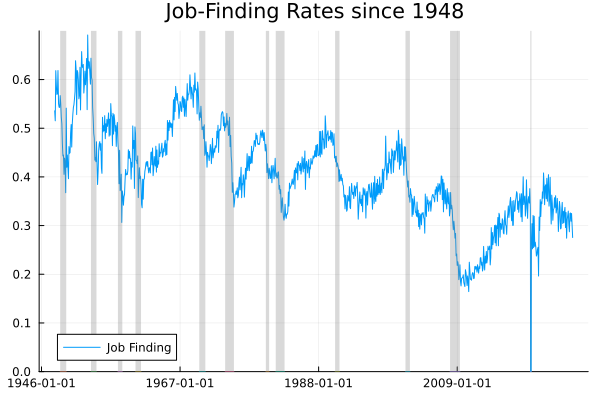
\includegraphics[scale=0.25]{fplot}
	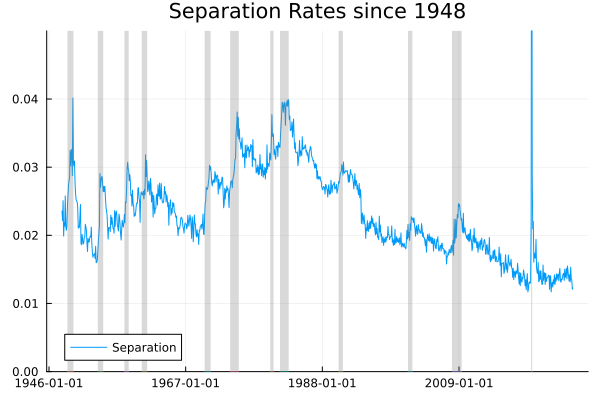
\includegraphics[scale=0.25]{splot}

	As expected, the data shows that the separation rate spikes at the start of recessions, while the job-finding rate drops over the course of the recession and then recovers. In this data, however, the separation rate appears to show a similar pattern, though less strongly. Since the year 2000, the imputed job-finding rate has noticeably dropped from its level in the 1900s; the mean appears to be about 0.05 to 0.1 lower.

	The imputed job-finding rate notably misses movements into and out of nonparticipation -- in particular, missing movements from employment to nonparticipation (due to, say, retirement) and movements from nonparticipation into unemployment (as a hedge against increased economic uncertainty). Whether this leads to the job-finding rate being overstated or understated depends on the specifics of the data: if \(N -> U\) movements are folded into \(u_{t+1}^s\), the job-finding rate will be overestimated during recessions, but if they are folded into \(u_{t+1}\), the job-finding rate will be underestimated during recessions.

	\subsection{The Flow Steady State}

	The computed steady-state unemployment is plotted against the actual unemployment rate below.

	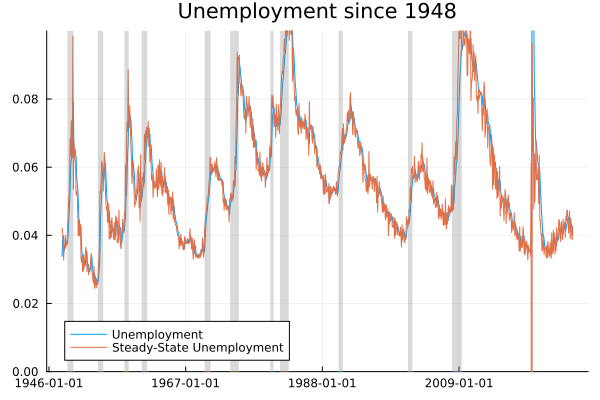
\includegraphics[scale=0.5]{unemploymentplot.png}

	The computed steady-state unemployment tracks the actual unemployment rate closely. This is mirrored in the sample means: the unemployment rate from the data is \(5.66\%\), while the computed steady-state unemployment rate is \(5.57\%\). We can see that the mean convergence factor is \(0.572\) months, while the half-life is \(-1.24\) months. This means that unemployment converges very quickly towards steady-state unemployment: it should make up more than half the difference in the space of two periods! Because the data follows this half-life, we should only expect there to be a significant gap between the steady-state unemployment and the actual unemployment during very large economic swings, and this is apparent in the data: the only obvious gaps are during the Great Recession of 2008 and the COVID-19 pandemic, which are also by far the largest swings in \(u\) in the data.

	\section{Theory}

	\subsection{McCall with Separation}

	\subsubsection{}

	We begin by writing the Bellman equations. Unemployed workers cannot separate from jobs, so their value function is exactly the same as in the base model:
	\[U = b + \beta \max_w\{E(w), U\} = b + \beta \left[ \int_{w^*}^{\bar{w}} E(w)\ dF(w) + \int_{\ubar{w}}^{w^*} U\ dF(w) \right]\] 
	The change in this model lies in the value function for the employed worker \(E(w)\), which is no longer the value of receiving \(w\) forever. It is now given by
	\[E(w) = w + \beta [(1 - \sigma) E(w) + \sigma U]\]
	which should remain constant for a given wage \(w\) since there is no renegotiation or on-the-job search. Since it is constant, we can rearrange for this value:
	\[ (1-\beta (1-\sigma)) E(w) = w + \beta \sigma U \implies E(w) = \frac{w + \beta \sigma U}{1-\beta(1-\sigma)}\]
	The reservation wage is the wage at which \(E(w^*) = U\), so we can also write
	\[ U = \frac{w^* + \beta \sigma U}{1 - \beta (1 - \sigma)} \implies (1-\beta (1-\sigma)) U = w^* + \beta \sigma U\]
	We can then see that
	\[ U - \beta U + \beta \sigma U - \beta \sigma U = w^* = (1 - \beta) U \implies U = \frac{w^*}{1 - \beta}\]
	which is exactly the same as in the original model! This is because the value of \(U\) does not depend directly on the separation probability; unemployed workers don't separate from jobs. The reservation wage encodes all the effects of the separation hazard.

	Now that we have solved for \(E\) and \(U\), we can solve for the reservation wage itself. Going back to the unemployed worker's Bellman equation, we now have:
	\[ \frac{w^*}{1 - \beta} = b + \beta \int_{w^*}^{\bar{w}} \frac{w + \beta \sigma \frac{w^*}{1 - \beta}}{1 - \beta (1 - \sigma)} dF(w) + \beta \int_{\ubar{w}}^{w^*} \frac{w^*}{1-\beta} dF(w) \]

	From this point we have no choice but to grind through algebra. We start by multiplying through by \(1-\beta\), then trying to get rid of the last integral term.
	\[ w^* \int_{\ubar{w}}^{w^*} dF(w) + w^* \int_{w^*}^{\bar{w}} dF(w) - \beta w^* \int_{\ubar{w}}^{w^*} dF(w) = (1 - \beta) b + \beta \int_{w^*}^{\bar{w}} \frac{w - \beta w + \beta \sigma w^*}{1 - \beta (1 - \sigma)} dF(w) \]
	Combining the lower integral terms on the left hand side, we get
	\[ (1 - \beta) w^* \int_{\ubar{w}}^{w^*} dF(w) + w^* \int_{w^*}^{\bar{w}} dF(w) = (1-\beta) b + \beta \int_{w^*}^{\bar{w}} \frac{w - \beta w + \beta \sigma w^*}{1 - \beta (1 - \sigma)} dF(w)        \]
	We then try to eliminate the integral on the left-hand side reservation wage term by splitting the upper integral. This gives us
	\begin{multline*}
	(1-\beta) \left( w^* \int_{\ubar{w}}^{w^*} dF(w) + w^* \int_{w^*}^{\bar{w}} dF(w)    \right) + \beta w^* \int_{w^*}^{\bar{w}} dF(w) \\= (1-\beta) b + \beta \int_{w^*}^{\bar{w}} \frac{w - \beta w + \beta \sigma w^*}{1 - \beta (1 - \sigma)} dF(w)
	\end{multline*}
	which simplifies to
	\[ (1 - \beta) w^* + \beta w^* \int_{w^*}^{\bar{w}} dF(w)= (1 - \beta) b + \beta \int_{w^*}^{\bar{w}} \frac{w - \beta w + \beta \sigma w^*}{1 - \beta (1 - \sigma)} dF(w)        \]
	Combining the remaining integrals gives us
	\[ (1-\beta)(w^* - b) = \beta \int_{w^*}^{\bar{w}} \frac{w - \beta w + \beta \sigma w^*}{1 - \beta (1 - \sigma)} - w^*  dF(w)      \]
	We now combine the terms under the integral into one fraction and get
	\[ (1 - \beta)(w^* - b) = \beta \int_{w^*}^{\bar{w}} \frac{w - \beta w + \beta \sigma w^* - w^* + \beta w^* - \beta \sigma w^*}{1 - \beta (1 - \sigma)} dF(w)        \]
	which simplifies to
	\[ (1 - \beta) (w^* - b) = \beta \int_{w^*}^{\bar{w}} \frac{w - \beta w - w^* + \beta w^* }{1 - \beta (1 - \sigma)} dF(w)   \]
	We can then pull out a \(1-\beta\) from the combined fraction, since it simplifies to 
	\[ (1-\beta) (w^* - b) = \frac{\beta}{1 - \beta (1 - \sigma)} \int_{w^*}^{\bar{w}} (1-\beta) w - (1 - \beta) w^*   dF(w)    \]
	And now the \(1 - \beta\) terms can divide out, giving us
	\[ w^* - b = \frac{\beta}{1 - \beta (1 - \sigma)} \int_{w^*}^{\bar{w}} (w - w^*) dF(w)    \]
	as required.

	\subsubsection{}

	To show the relationship between \(w^*\) and \(\sigma\), we will need to use the implicit function theorem. Taking partial derivatives, we get
	\[ \frac{\partial w^*}{\partial \sigma} = - \left( \frac{\beta}{1 - \beta (1 - \sigma)} \right)^2 \int_{w^*(\sigma)}^{\bar{w}} (w - w^*(\sigma) dF(w) - \frac{\beta}{1 - \beta (1 - \sigma)} (1 - F(w^*(\sigma))) \frac{\partial w^*}{\partial \sigma}  \]
	Let's simplify this by writing \(g(\sigma) = 1 - \beta (1 - \sigma)) = 1 - \beta + \beta \sigma\). That gives us 
	\[ \frac{\partial w^*}{\partial \sigma} = - \left( \frac{\beta}{g(\sigma)} \right)^2 \int_{w^*(\sigma)}^{\bar{w}} (w - w^*(\sigma) dF(w) - \frac{\beta}{g(\sigma)} (1 - F(w^*(\sigma))) \frac{\partial w^*}{\partial \sigma}  \]
	We combine the partial derivative terms to get
	\[ \left( \frac{g(\sigma) + \beta (1 - F(w^*(\sigma)))}{g(\sigma)}     \right) \frac{\partial w^*}{\partial \sigma} = - \left( \frac{\beta}{g(\sigma)} \right)^2 \int_{w^*(\sigma)}^{\bar{w}} (w - w^*(\sigma) dF(w)      \]
	Then we isolate the partial derivative.
	\[ \frac{\partial w^*}{\partial \sigma} = - \left( \frac{\beta^2 g(\sigma)}{g(\sigma)^2 (g(\sigma) + \beta (1 - F(w^*(\sigma))))} \right) \int_{w^*(\sigma)}^{\bar{w}} (w - w^*(\sigma) dF(w)      \]
	which simplifies to 
	\[ \frac{\partial w^*}{\partial \sigma} = - \left( \frac{\beta^2}{g(\sigma) (g(\sigma) + \beta (1 - F(w^*(\sigma))))} \right) \int_{w^*(\sigma)}^{\bar{w}} (w - w^*(\sigma) dF(w)      \]

	We can see that \(g(\sigma) = 1 - \beta (1 - \sigma)\) is positive since \(\beta\) and \(\sigma\) lie in \([0,1]\). \(F(w^*(\sigma))\) must also lie in \([0,1]\) since it is a probability function, so the term in parentheses must be positive. The term under the integral also must be positive since \(w\) is always above \(w^*\) in this integral. Thus this expression for \(\frac{\partial w^*}{\partial \sigma}\) must be negative since it is the negative of the product of two positive quantities. 

	The partial derivative being negative means that the reservation wage goes down when the separation rate rises. Directly, this means that a worker is willing to accept a lower wage for a job when she is more likely to lose that job. Effectively, the separation risk means that she is also no longer 'locked in' to a particular wage draw: even if the worker gets a wage offer lower than she might like otherwise, she can always take the wage offer, wait for separation to hit, then redraw a better offer. She is no longer giving up as much in future earnings as she would in the world of the original McCall model, where she would be locked into her low draw forever. 
	
	However, while there is a world where the worker could end up searching for a better job, we can also derive an additional implication from this model: the worker is made worse off by the existence of job separation. Because \( w^* = U\), we know that \(\frac{\partial U(w(\sigma))}{\partial \sigma} < 0\), so the worker is ultimately made worse off when she can lose a job.

	\subsubsection{}

	We let \(F\) be uniform on \([0,1]\). We can immediately rewrite the wage equation as
	\[ w^* - b = \frac{\beta}{1 - \beta (1 - \sigma)} \int_{w^*}^{1} (w - w^*) \frac{1}{1 - 0} dw = \frac{\beta}{1 - \beta (1 - \sigma)} \int_{w^*}^{1} (w - w^*) dw   \]
	The integral is now solveable by hand:
	\[  \int_{w^*}^{1} (w - w^*) dw = \Bigg[\frac{1}{2} w^2 - w^* w \Bigg]_{w = w^*}^{w = 1} = \frac{1}{2} - w^* - \frac{1}{2} (w^*)^2 + (w^*)^2 = \frac{1}{2} - w^* + \frac{1}{2}(w^*)^2\]
	This then gives lets us rewrite the initial equation as 
	\[ w^* - b = \frac{1}{2}\Bigg(\frac{\beta}{1 - \beta (1 - \sigma)}\Bigg) \Bigg( 1 - 2w^* + (w^*)^2 \Bigg) = \frac{1}{2}\Bigg(\frac{\beta}{1 - \beta (1 - \sigma)}\Bigg) \Bigg( w^* - 1 \Bigg)^2  \]
	Let us write \(C = \frac{1}{2}\frac{\beta}{1 - \beta (1 - \sigma)}\) to make this easier to read. This becomes
	\[ w^* - b = C \Big((w^*)^2 - 2w^* + 1\Big) \implies C(w^*)^2 - (2C - 1) w^* + (C + b) = 0     \]

	[insert computations]

	Now we force \( \lambda = \bar{s} = 0.40444  \). This immediately gives \(w^* = 1 - 0.40444 = 0.59556\). Assuming \(\sigma = 0.02\), we can rework the model to be
	\[ b = -C*[w^* - 1)^2 - w^*]     \] 
	Calculating through, we see that this model requires \(b\) to be close to \(0.7\), more than twice our calibration! This suggests 
	
	\subsection{The wage equation, in and out of steady state}

	\subsubsection{}

	We will start by assuming that all of \(w\), \(b\), and \(\kappa\) could vary to get a more general model. Matches between firms and workers are created by a Cobb-Douglass matching technology:
	\[ M(u,v) = \chi u^\eta v^{1-\eta}    \]
	which gives job-finding probabilities
	\begin{align*}
	\lambda_w(\theta) &= \frac{M(u,v)}{u} = \chi \theta^{1-\eta} \\
	\lambda_f(\theta) &= \frac{M(u,v)}{v} = \chi \theta^{-\eta}
	\end{align*}
	and immediately gives the relationship \(\lambda_w = \theta \lambda_f\). Next we  write down the value functions for (un)employed workers and both vacant and filled jobs.
	\begin{align*}
	U(b) &= b + \beta \left[\lambda_w(\theta) W(w') + (1 - \lambda_w(\theta)) U(b')\right]\\
	W(w) &= w + \beta \left[(1 - \sigma) W(w') + \sigma U(b')\right]\\
	V(\kappa) &= - \kappa + \beta \left[\lambda_f(\theta) J(w') + (1 - \lambda_f(\theta)) V(\kappa')\right]\\
	J(w) &= z - w + \beta \left[(1-\sigma) J(w') + \sigma V(\kappa')\right]
	\end{align*}
	Using these Bellman equations, we can define the joint surplus:
	\[ S(w) = \Big(W(w) - U(w)\Big) + \Big(J(w) - V(w)\Big)     \]
	Now we need to solve the bargaining problem. This is expressed as
	\[ w = \arg \max \left\{\Big(W(w)-U(b)\Big)^\gamma \Big(J(w) - V(\kappa)\Big)^{1-\gamma}\right\}  \]
	which has first order condition
	\begin{multline*}
	\gamma \Big(W(w) - U(b)\Big)^{\gamma - 1}W' \Big(J(w) - V(\kappa)\Big)^{1-\gamma} \\+ (1 - \gamma) \Big(J(w) - V(\kappa)\Big)^{-\gamma} J'(w) \Big(W(w) - U(b)\Big)^{\gamma} = 0
	\end{multline*}
	Looking at the equations for \(W(w)\) and \(J(w)\), we see that they are linear, so we can replace their derivatives with \(1\) and \(-1\), respectively. This lets us rearrange the first-order condition to
	\[ \gamma J(w) = (1 - \gamma)\Big(W(w) - U(b)\Big)   \]
	At this point we impose the free entry condition to set \(V = 0\). Then we can replace these conditions with our Bellman equations:
	\[ \gamma \Bigg( z - w + (1 - \sigma) \beta J(w')\Bigg) = (1 - \gamma) \Bigg( w - b + (1 - \sigma - \lambda_w(\theta)) \beta \Big[   W(w') - U(b')\Big]  \Bigg)    \]
	The right hand side can also be rewritten in terms of \(J(w) - V(\kappa)\):
	\[ \gamma \Bigg( z - w + (1 - \sigma) \beta J(w') \Bigg) = (1 - \gamma) \Bigg( w - b + (1 - \sigma - \lambda_w(\theta)) \frac{\gamma}{1 - \gamma}\beta J(w')  \Bigg)    \]
	Now we just have to worry about \(J(w')\)! And we can solve for this with the vacancy equation:
	\[ V(\kappa) = 0 = -\kappa + \beta \Big[ \lambda_f(\theta) J(w') + 0 \Big] \implies J(w') = \frac{\kappa}{\beta \lambda_f(\theta)}  \]
	This in turn lets us substitute out \(J(w')\) in the equation above:
	\[ \gamma \Bigg(z - w + (1 - \sigma) \beta \frac{\kappa}{\beta \lambda_f(\theta)}\Bigg) = (1 - \gamma)\Bigg(w - b + (1 - \sigma - \lambda_w(\theta)) \frac{\gamma}{1 - \gamma} \beta \frac{\kappa}{\beta \lambda_f(\theta)}\Bigg)     \]
	This allows the \(\beta\)s to cancel:
	\[ \gamma (z - w) + \gamma \frac{\kappa (1 - \sigma)}{\lambda_f(\theta)} = (1 - \gamma)(w - b) + \gamma \frac{(1 - \sigma - \lambda_w(\theta)) \kappa}{\lambda_f(\theta)}   \]
	We can also rewrite the first terms slightly to get
	\[ \gamma z + \gamma \frac{\kappa (1 - \sigma)}{\lambda_f(\theta)} = w - (1 - \gamma) b + \gamma \frac{(1 - \sigma - \lambda_w(\theta)) \kappa}{\lambda_f(\theta)}    \]
	Rearranging this equation, we have
	\[ w = (1 - \gamma) b + \gamma z + \gamma \kappa \frac{1 - \sigma - 1 + \sigma + \lambda_w(\theta)}{\lambda_f(\theta)}  \]
	which simplifies to
	\[ w = (1 - \gamma) b + \gamma z + \gamma \kappa \frac{\lambda_w(\theta) }{\lambda_f(\theta)}    \]
	at which point we can substitute \(\lambda_w(\theta) = \theta \lambda_f(\theta)\) and get
	\[ w = (1 - \gamma) b + \gamma (z + \kappa \theta)  \]
	like we want. 
	
	Now we want to derive an equation for the surplus itself. We again want to obtain an equation in \(J(w')\). We start by deriving \(W - U\) as a fraction of the surplus. The first-order condition says 
	\[ S = \Big(W(w) - U(b)\Big) + \Big(J(w) - V(\kappa)\Big)  \]
	Imposing free entry and then substituting the Bellman equations, we get
	\[ S = w - b + z - w + \beta \bigg[ (1 - \sigma - \lambda_w(\theta)) \Big(W(w') - U(b')\Big) + (1 - \sigma) J(w') \bigg]     \]
	This time, we want to solve for \(S\). We replace \(W - U\) and \(J\) with their associated fractions of the surplus:
	\[ S = z - b + \beta \bigg[ (1 - \sigma - \lambda_w(\theta)) \gamma S  + (1 - \sigma) (1 - \gamma) S \bigg]     \]
	Expanding the various terms in parentheses, we have
	\[ S = z - b + S \Big( \gamma \beta - \gamma \beta \sigma - \gamma \beta \lambda_w(\theta) + \beta - \beta \sigma - \beta \gamma + \beta \gamma \sigma   \Big)    \]
	which simplifies to 
	\[ S = z - b + S \Big( \beta - \gamma \beta \lambda_w(\theta) - \beta \sigma   \Big) = z - b + \beta S \Big( (1 - \sigma) - \gamma \lambda_w(\theta)   \Big)    \]
	Combining the S terms, we get
	\[ 1 -  \beta \Big( (1 - \sigma) - \gamma \lambda_w(\theta)   \Big) S = z - b \]
	and thus derive the equation for the surplus
	\[ S = \frac{z - b}{1 -  \beta (1 - \sigma) + \beta \gamma \lambda_w(\theta)} \]
	as required. 
	\subsubsection{}

	The above derivation intentionally avoided imposing the steady-state condition when deriving the equations for the surplus and wage equation; thus, it should be evident that they will hold even if the economy is not in steady state provided the economy is in equilibrium.

	\subsubsection{}

	\section{Computation}

	\subsection{Calibrate to your hazards}
	The model boils down to solving
	\[     \]
	\subsection{Comparative statics}

	\subsection{The Beveridge loop}

\end{document}